\section{Experiments}\label{sec:experiments}

The bounds in Theorems~\ref{thm:one-round}, \ref{thm:multi-round}, and~\ref{thm:var-pp} predict that, holding the clip \(C\) and the noise scale \(\sigma\) fixed, the per-client memorization \(I(X_k;\transcript\mid P)\) decays like \(O(1/K^2)\) as the number of clients \(K\) grows. We do not estimate the conditional mutual information directly---high-dimensional CMI estimation is itself a hard problem---and instead measure a standard operational proxy: the per-client \emph{train--test accuracy gap} on long-tailed data. This proxy is a lower bound on memorization in the sense that an algorithm that fits its training set strictly better than a fresh test set drawn from the same conditional distribution must have used some information about the realized training set beyond what \(P\) implies, and hence must have nonzero conditional mutual information about \(X_k\).

\subsection{Setup}\label{sec:exp-setup}

\paragraph{Data.} We use the long-tailed image-classification benchmark introduced as a memorization stress test by \citet{Brown2021Memorization}. Concretely, we take 50 classes from Tiny-ImageNet \citep{Le2015TinyImageNet} and assign per-class training counts that decay exponentially from 500 (head) to 5 (tail), giving \(n=5\,522\) training images and \(2\,500\) held-out test images (50 per class). The exponential schedule means roughly half the classes have under 50 examples each, which is the regime in which Brown et al.\ predict heavy memorization is unavoidable for accurate classifiers.

\paragraph{Federated partition.} For each \(K\in\{1,2,4,6,8,10\}\) we partition the long-tailed dataset across clients with a Dirichlet distribution: for each class \(c\), draw \(p_c\sim\mathrm{Dirichlet}(\alpha,\dots,\alpha)\in\Delta^{K-1}\) with \(\alpha=0.5\) and split that class's training and test indices across clients in proportion \(p_c\). The per-class proportions are shared between train and test, so each client receives an i.i.d.\ pair (train\(_k\), test\(_k\)) drawn from a client-specific class mixture; this matches the i.i.d.\ generative model of Assumption~\ref{ass:indep} at the client level. The partition is heterogeneous in the standard non-IID-FL sense: at \(K=10\), most clients see only a handful of classes with appreciable mass.

\paragraph{Model and optimizer.} We train a ResNet-18 \citep{He2016ResNet} with batch normalization replaced by group normalization (8 groups), so that all model state is captured by \(\theta\) and transmitted through \(\mathrm{flat\_params}(\theta)\) at each round; this is the configuration recommended by \citet{Hsieh2020NonIID} for federated training. Clients run two local epochs of stochastic gradient descent (mini-batch size 64, learning rate 0.1, momentum 0.9, weight decay \(5\times 10^{-4}\)) on \(X_k\) starting from the broadcast iterate \(\theta^{(t)}\), and return the local delta \(V_k^{(t)}=\theta_k^{\mathrm{local}}-\theta^{(t)}\). The server clips each \(V_k^{(t)}\) to Euclidean norm \(C=10\), averages, and adds isotropic Gaussian noise of scale \(\sigma=3\times 10^{-4}\). All runs use the same seed and the same long-tailed class subset; the only varying parameter is \(K\). We train for \(T=40\) rounds and evaluate per-client per-class train and test accuracy at the end of training.

\paragraph{Hardware and runtime.} A single sweep over \(K\in\{1,\dots,10\}\) completes in roughly 37 minutes on one A100 40\,GB GPU.

\subsection{Results}\label{sec:exp-results}

\paragraph{Community-level memorization gap.} Figure~\ref{fig:summary-vs-K} plots the average train and test accuracy on the head 20\% of classes (high-frequency) and the tail 20\% (low-frequency), together with the corresponding train--test gap, as a function of \(K\). At \(K=1\) (centralized, single-client DP-SGD), the model attains 98\% train accuracy on head classes and 48\% on tail classes, while test accuracy is 54\% (head) and \(\approx 0\)\% (tail)---the classic signature of memorization on rare classes. As \(K\) grows, the gap collapses: at \(K=10\), head-class train and test accuracy both lie near 32\% (gap \(\approx 1\) point), and tail-class train accuracy itself collapses to zero. Memorization on rare classes is the first thing the averaging mechanism erases.

\begin{figure}[h]
\centering
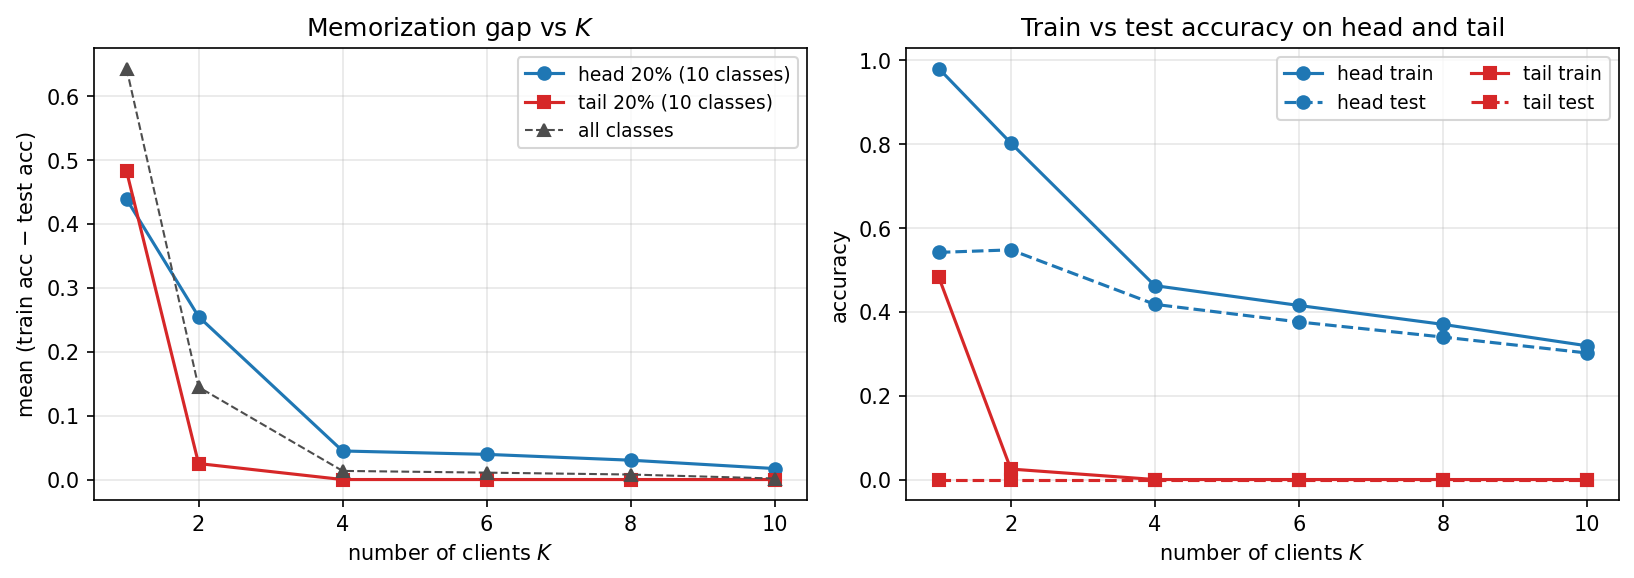
\includegraphics[width=\linewidth]{figures/fig3_summary_vs_K.png}
\caption{Community-level memorization gap as a function of the number of clients \(K\), holding the clip bound \(C=10\) and noise scale \(\sigma=3\times 10^{-4}\) fixed. \textbf{Left:} mean train--test gap on head 20\% of classes (blue), tail 20\% (red), and across all 50 classes (gray). \textbf{Right:} train (solid) versus test (dashed) accuracy on head and tail classes. The monotone collapse of the gap from \(\sim\)44 percentage points (head) and \(\sim\)48 (tail) at \(K=1\) to \(\le 1\) at \(K=10\) is consistent with the \(O(1/K^2)\) per-client memorization bound of Theorem~\ref{thm:multi-round}.}
\label{fig:summary-vs-K}
\end{figure}

\paragraph{Per-client memorization gap.} Figure~\ref{fig:per-client-box} shows the distribution across clients of per-client train accuracy, test accuracy, and train--test gap, for each \(K\). The gap distribution shrinks monotonically with \(K\): median gap drops from 75 percentage points at \(K=1\) to \(\approx 15\) at \(K=10\), with inter-client variance also tightening. At \(K=10\) every individual client has a train--test gap below 30 points, compared to gaps in excess of 70 points for the centralized run.

\begin{figure}[h]
\centering
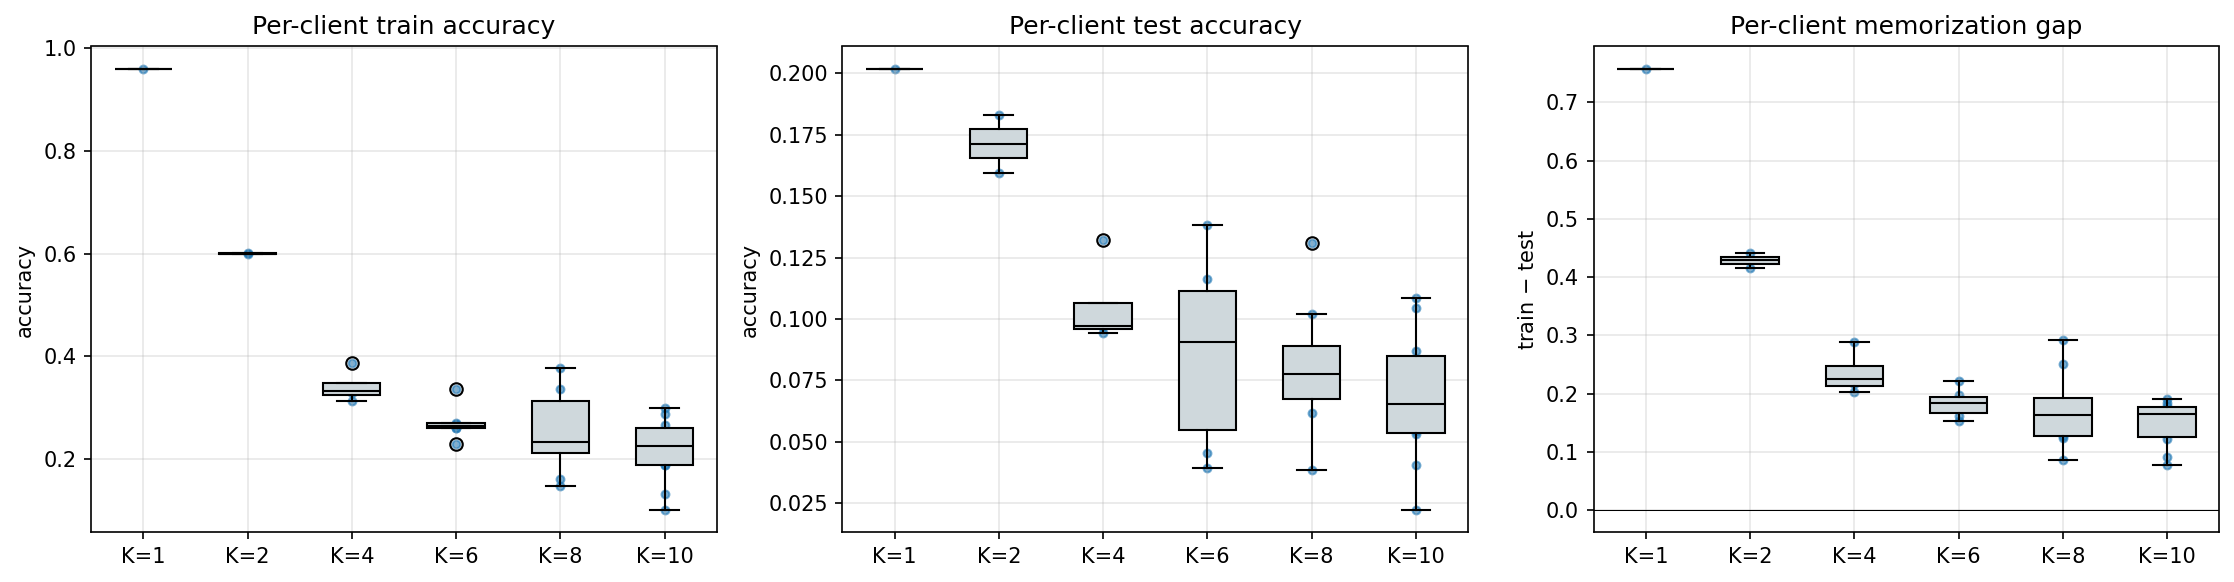
\includegraphics[width=\linewidth]{figures/fig6_per_client_box.png}
\caption{Per-client distributions of train accuracy (left), test accuracy (middle), and train--test gap (right), as a function of \(K\). Each box aggregates over the \(K\) clients in that run. The per-client gap distribution shrinks monotonically with \(K\), consistent with the per-client bound \(I(X_k;\transcript\mid P)=O(1/K^2)\).}
\label{fig:per-client-box}
\end{figure}

\paragraph{Per-class detail at \(K=10\).} Figure~\ref{fig:client-heatmap} gives a per-client per-class view at \(K=10\): one row per client, one column per class (sorted from head to tail; gray cells indicate classes the client did not own). The rightmost panel, the train--test gap, is near-uniformly white (gap close to zero) across both head and tail classes, confirming that at \(K=10\) the residual memorization signal on individual clients is essentially gone and that the residual head-class accuracy seen in Figure~\ref{fig:summary-vs-K} comes from generalizable structure, not from fitting individual rare examples.

\begin{figure}[h]
\centering
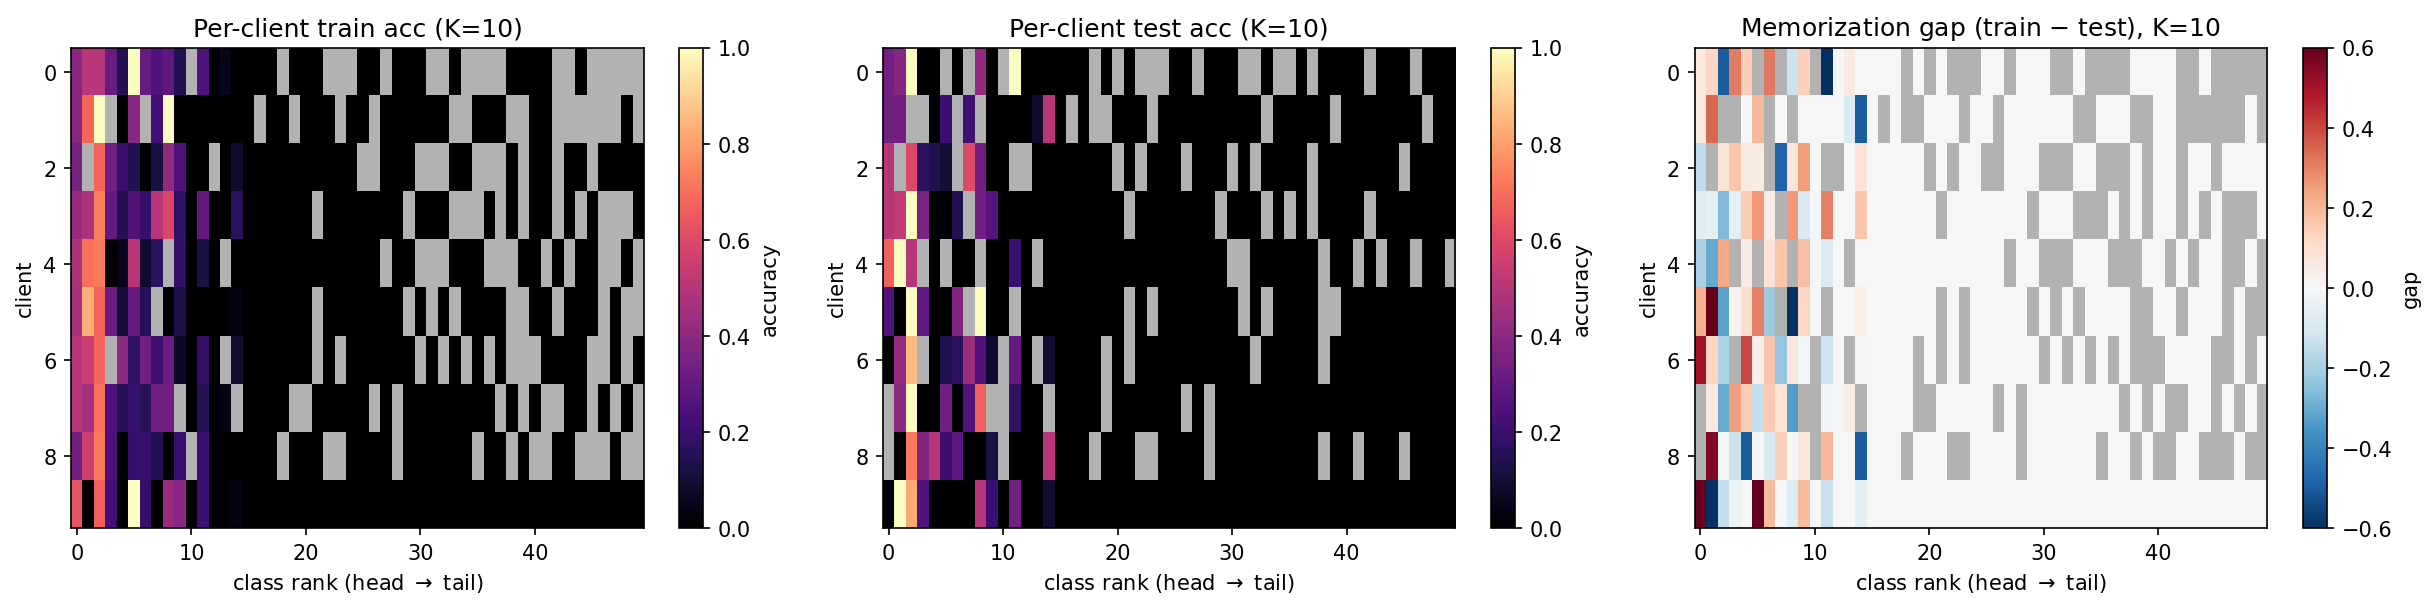
\includegraphics[width=\linewidth]{figures/fig4_client_heatmap.png}
\caption{Per-client, per-class breakdown at \(K=10\): train accuracy (left), test accuracy (middle), and train--test gap (right). Rows index clients, columns index classes (sorted head\(\to\)tail). Gray cells mark classes that a given client did not receive in its Dirichlet partition. The gap panel is near-uniformly white, indicating that the per-client memorization signal has collapsed.}
\label{fig:client-heatmap}
\end{figure}

\paragraph{Caveats.} The train--test gap is a lower-bound proxy, not a direct estimator of \(I(X_k;\transcript\mid P)\); a small empirical gap is consistent with both small CMI and with a model that has memorized but failed to retrieve at evaluation time. The experiment also operates at a noise scale (\(\sigma=3\times 10^{-4}\)) far below what a deployed DP-FedAvg system would use---this was chosen so that the centralized \(K=1\) baseline could exhibit the strong memorization predicted by \citet{Brown2021Memorization} and that our bound then collapses; the qualitative \(K\)-dependence of the gap is the comparison of interest, not the absolute privacy level. Finally, the bound concerns the transcript \(\transcript\) (or by post-processing the final iterate \(\theta^{(T)}\)); we treat the trained model's behavior on training versus test inputs as a downstream proxy.
